\documentclass[tikz]{standalone}
\usepackage{helvet}
\usepackage[T1]{sansmath}
\renewcommand{\familydefault}{\sfdefault}
\normalfont

\begin{document}
\begin{sansmath}

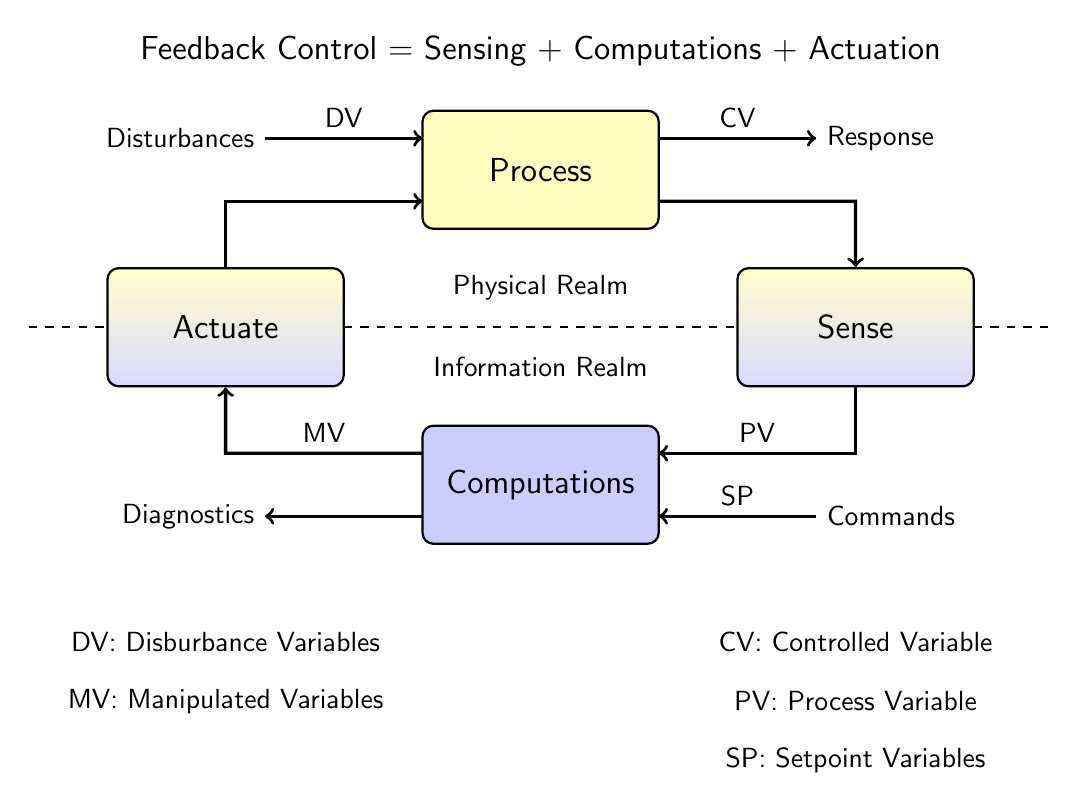
\begin{tikzpicture}[
        auto,
        block/.style = {rectangle, draw, thick, 
        rounded corners, minimum height = 1.5cm, minimum width = 3cm},
        thick]
    %\draw [help lines] (0,-3) grid (14,7);
    
    \shade [top color = yellow!20, bottom color = blue!15, rounded corners]
     (1.5,2.25) rectangle ++(3,1.5);

    \shade [top color = yellow!20, bottom color = blue!15, rounded corners]
     (9.5,2.25) rectangle ++(3,1.5);
        
    \node [block,fill=yellow!25] (process) at (7,5) {\large Process};
    \node [block,fill=blue!20] (control) at (7,1) {\large Computations};
    \node [block] (sensor) at (11,3) {\large Sense};   
    \node [block] (actuator) at (3,3) {\large Actuate};
    
    \draw [dashed] (.5,3) -- (1.5,3) ++ (3,0) -- ++(5,0) ++ (3,0) -- ++(1,0);
    \draw [->,very thick] (control) ++ (-1.5,0.4) --
        node[midway,above] {MV} ++ (-2.5,0) -- (actuator);
    \draw [->,very thick] (actuator) -- ++(0,1.6) -- ++(2.5,0);
    \draw [->,very thick] (process) ++ (1.5,-0.4) -- ++(2.5,0) -- (sensor);
    \draw [->,very thick] (sensor) -- ++(0,-1.6) --
        node[midway,above] {PV} ++ (-2.5,0);
    
    \draw [<-,very thick] (process) ++(-1.5,0.4) -- 
        node[midway,above] {DV} ++(-2,0) node[left] {Disturbances};
    \draw [<-,very thick] (control)  ++(1.5,-0.4) --
        node[midway,above] {SP} ++ (2,0) node[right] {Commands};
    \draw [->,very thick] (process) ++ (1.5,0.4) --
        node [midway,above] {CV} ++(2,0) node[right] {Response};
    \draw [->,very thick] (control) ++ (-1.5,-0.4) -- ++(-2,0)
        node[left] {Diagnostics};
    
    \node at (7,3.5) {Physical Realm};
    \node at (7,2.5) {Information Realm};
    \node at (7,6.5) {\large Feedback Control = Sensing + Computations + Actuation};
    
   	\node at (11,-1) {CV: Controlled Variable};
   	\node at (11,-1.75) {PV: Process Variable};   	
   	\node at (11,-2.5) {SP: Setpoint Variables};
   	\node at (3,-1) {DV: Disburbance Variables};
   	\node at (3,-1.75) {MV: Manipulated Variables};
   	
    
\end{tikzpicture}

\end{sansmath}
\end{document}
